\documentclass{beamer}
\usepackage[orientation=landscape,size=a0,scale=1.4]{beamerposter}
\mode<presentation>{\usetheme{LAS}}
\usepackage[utf8]{inputenc}
\usepackage[english]{babel}
\usepackage{hyperref} %enable hyperlink for urls
\usepackage{ragged2e}
\usepackage{calc}
\usepackage{xcolor}
\usepackage{multicol}
\setlength{\columnsep}{-4cm}
\newlength{\mylength}

\usepackage{array,booktabs,tabularx}
\newcolumntype{Z}{>{\centering\arraybackslash}X} % centered tabularx columns

\title{\huge The Magic of Specifications and Type Systems}
\author{Amin Bandali, Simon Hudon, Jonathan Ostroff}
\institute[York University]{Software Engineering Lab, EECS}
\date{August 18, 2016}

\newlength{\columnheight}
\setlength{\columnheight}{74cm}

\newcommand{\tla}{TLA${}^+$}

\begin{document}
\begin{frame}
\begin{columns}
  \begin{column}{.3\textwidth}
    \begin{beamercolorbox}[center]{postercolumn}
      \begin{minipage}{.98\textwidth} % tweaks the width, makes a new \textwidth
        \parbox[t][\columnheight]{\textwidth}{ % must be some better way to set
                                               % the the height, width and
                                               % textwidth simultaneously
          \begin{myblock}{Introduction}
            \begin{itemize}
              \item Architects draw detailed plans before a brick is laid or a
                nail is hammered. Programmers and software engineers don't.
                \textit{Can this be why houses seldom collapse and programs
                  often crash?}

              \item Blueprints help architects ensure that what they are
                planning to build will work. ``Working'' means more than not
                collapsing; it means serving the required purpose. Architects
                and their clients use blueprints to understand what they are
                going to build before they start building it.

              \item But few programmers write even a rough sketch of what their
                programs will do before they start coding.

              \item \textbf{Specifications}: To designers of complex systems,
                the need for formal specifications should be as obvious as the
                need for blueprints of a skyscraper. But few software
                developers write \textit{specifications} because they have
                little time to learn how on the job, and they are unlikely to
                have learned in school. Some graduate schools teach courses on
                specification languages, but few teach how to use specification
                in practice. It's hard to draw blueprints for a skyscraper
                without ever having drawn one for a toolshed.
            \end{itemize}
            [\textit{Leslie Lamport, Turing Award Winner, 2013}]
            \bigskip

            Specifications (and formal methods) used to be relegated to safety
            critical systems like nuclear power, avionics and medical devices.
            Increasingly, a variety of industrial strength formal methods (e.g.
            \tla~\cite{DBLP:books/aw/Lamport2002},
            Event-B~\cite{DBLP:books/daglib/0024570}, and many others) are now
            being used by Microsoft, Amazon, Facebook and Dropbox.
          \end{myblock}

          \begin{myblock}{Significance \& Contributions}
            {Unit-B}~\cite{SoSyM/Hudon/Hoang/Ostroff15} is a new framework for
            specifying and modelling systems that must satisfy both safety and
            liveness properties.Compared to Event-B, Unit-B brings in record
            types and complete well-definedness. In comparison to \tla, Unit-B
            adds type checking, well-definedness checking and quantification
            over infinite sets.
            \bigskip

            \textbf{Unit-B Web} makes the Literate Unit-B prover available on
            the web. Unit-B Web leverages the automated predicate prover to
            two purposes:

            \begin{itemize}
              \item \textbf{Teaching}: can be used in classroom for
                demonstrations, or in evaluation in the form of online quizzes.

              \item \textbf{Online Proof Environment}, making specifications
                more accessible to casual users. It also serves as a ``proof of
                concept'' for a web IDE for the full modelling capabilities of
                Unit-B.
            \end{itemize}
            \bigskip

            Unit-B Web's technology stack:
            $\bullet$ {Syntax:} based on \LaTeX\
            $\bullet$ {Web:} JavaScript, JSON, Yesod / Haskell
            $\bullet$ {Prover:} Haskell, Z3

          \end{myblock}\vfill
    }\end{minipage}\end{beamercolorbox}
  \end{column}
  \begin{column}{.4\textwidth}
    \begin{beamercolorbox}[center]{postercolumn}
      \begin{minipage}{.98\textwidth}  % tweaks the width, makes a new \textwidth
        \parbox[t][\columnheight]{\textwidth}{ % must be some better way to set the the height, width and textwidth simultaneously
          \begin{myblock}{Unit-B Web Snapshot}
            Below are two screenshots of the Unit-B Web tool, showcasing its
            type checking and well-definedness checking capabilities.

            \begin{figure}
              \centering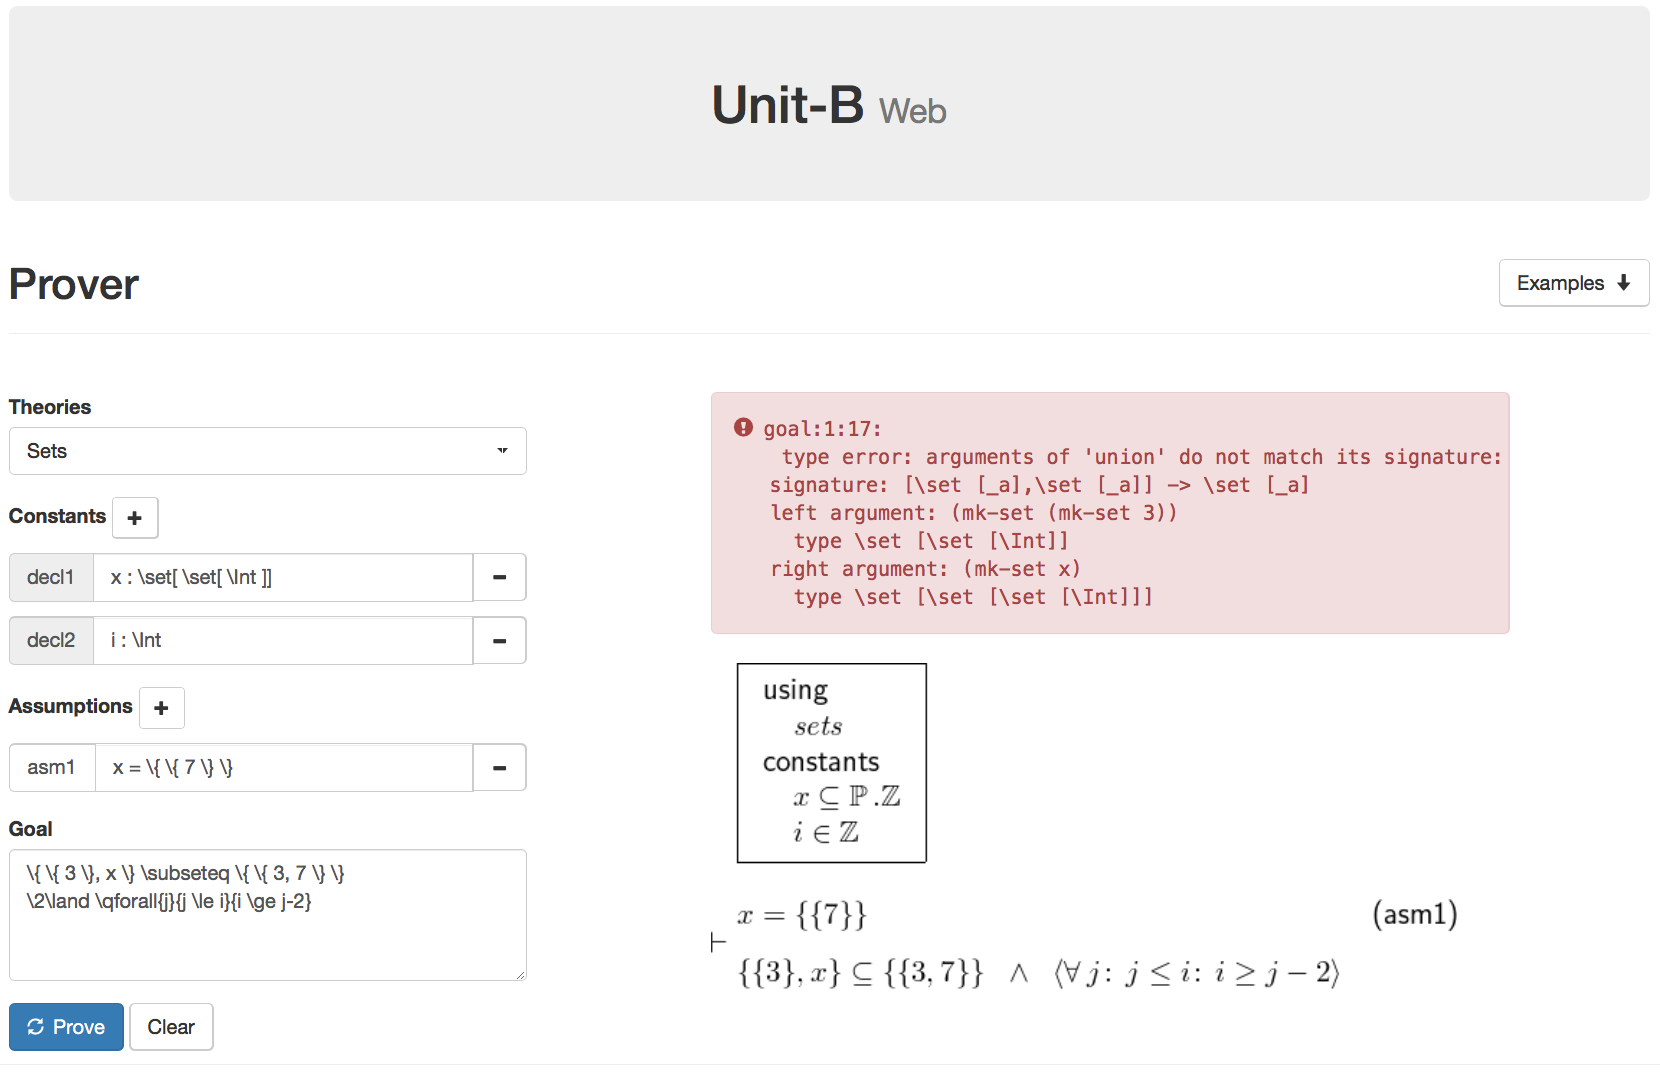
\includegraphics[width=\textwidth]{img/unitb-example1.png}
              \caption{A type error --- $x$ is expected to be a set of
                numbers}\label{fig:typechecking}
            \end{figure}
          \end{myblock}
          \begin{myblock}{Unit-B Web Snapshot}
            \begin{figure}
              \begin{minipage}{0.94\textwidth}
                \centering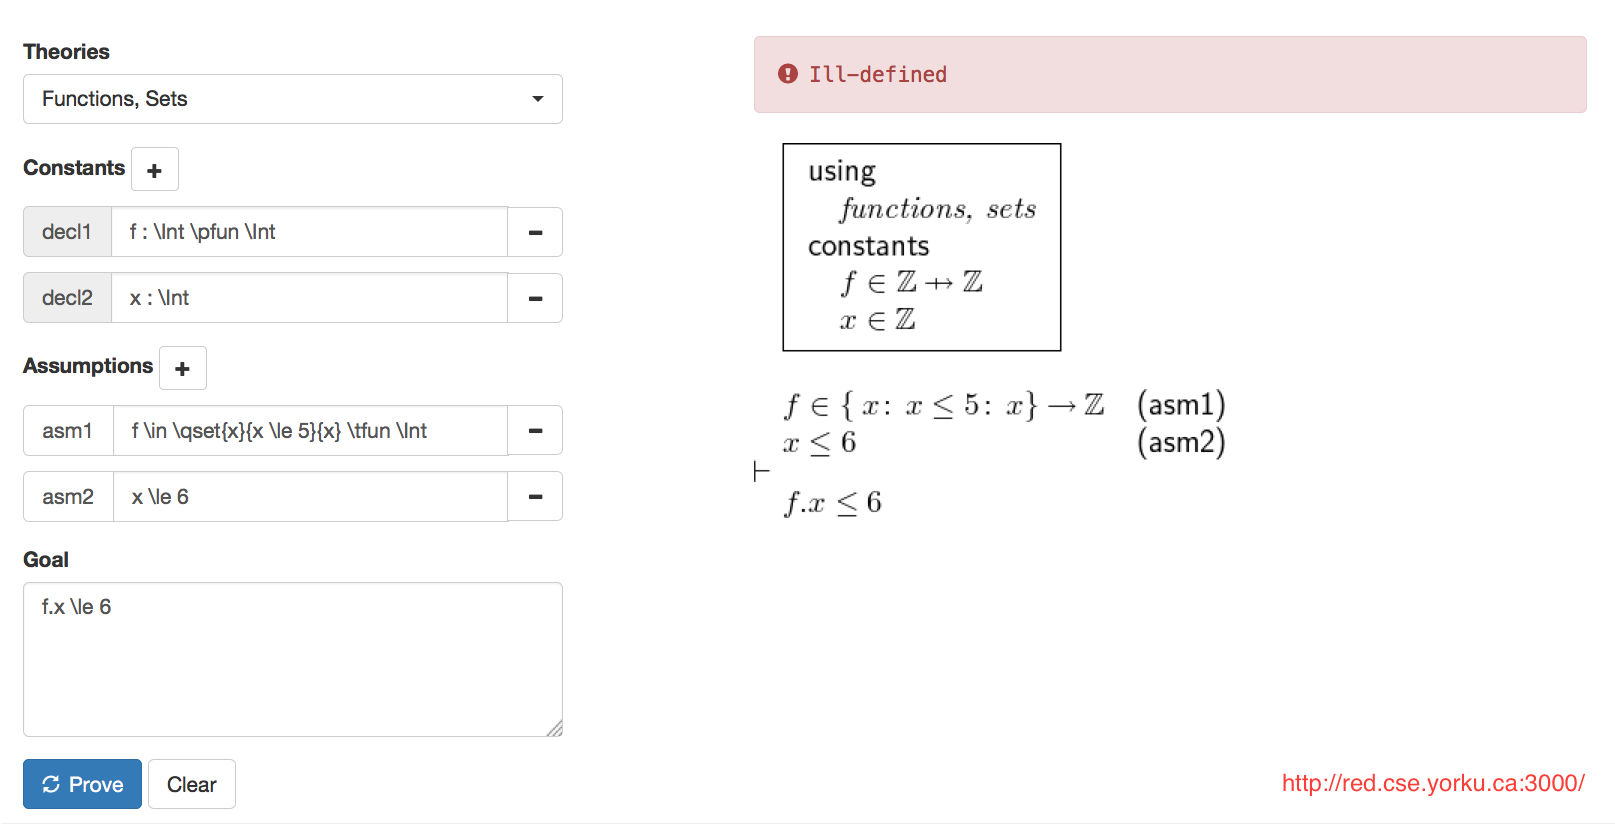
\includegraphics[width=\textwidth]{img/unitb-example2.png}
                \caption{An ill-defined predicate --- $x$ is not in
                  the domain of $f$}\label{fig:wd}
              \end{minipage}
            \end{figure}
          \end{myblock}\vfill
    }\end{minipage}\end{beamercolorbox}
  \end{column}
  \begin{column}{.3\textwidth}
    \begin{beamercolorbox}[center]{postercolumn}
      \begin{minipage}{.98\textwidth} % tweaks the width, makes a new \textwidth
        \parbox[t][\columnheight]{\textwidth}{ % must be some better way to set
                                               % the the height, width and
                                               % textwidth simultaneously
          \renewcommand{\figurename}{Fig.}
          \begin{myblock}{Type Checking}
            Some formulas, such as $\{x\} + 3 \le 7$, are not meaningful. Type
            checking helps us identify and fix them instead of laboring
            needlessly over the proof of meaningless formulas. \tla\ does not
            recognize this as an error; Unit-B does (see
            \figurename~\ref{fig:typechecking}).
            \bigskip

            \tla\ is an untyped logic which allows expressive formulas such as
            $\{ 3, \{ 7 \} \}$. In a simple type system such as that of Event-B,
            homogeneity rules out such a formula. The challenge in a typed
            system such as Unit-B is to allow such formulas. We do this using
            subtyping.
            \bigskip

            Further, type variables in Unit-B allow for polymorphic definitions,
            e.g.\ using the same functions on sets of numbers and sets of sets
            of numbers.\newline
            \vspace{-1em}
          \end{myblock}
          \begin{myblock}{Well-definedness Checking}
            WD checking~\cite{DBLP:conf/cade/DarvasMR08} catches meaningless
            formulas that the type checker cannot catch, such as division by
            zero or array out of bounds.
            \bigskip

            Unit-B's WD-calculus is complete; while Event-B's is incomplete.
            Let us consider the following example with four propositions
            $A$, $B$, $C$, and $D$ (which we will specify shortly), where

            \vspace{-3ex}
            \begin{eqnarray*}
              A \Rightarrow WD(B) \\
              B \Rightarrow WD(C) \\
              B \Rightarrow WD(D)
            \end{eqnarray*}

            The following calculation is not well-defined in Event-B (the
            {\color{red}red} formula is rejected), but it is well-defined
            in Unit-B:\

            \vspace{-2ex}
            \begin{multicols}{2}
              \begin{align*}
                & A \wedge B \wedge (C \vee D) \\
                = \ & \{ \textit{associativity} \} \\
                & {\color{red} A \wedge (C \vee D) \wedge B} \\
                = \ & \{ \textit{distributivity} \} \\
                & ( (A \wedge C) \vee (A \wedge D) ) \wedge B
              \end{align*}
              \columnbreak\
              \begin{align*}
                \\[-1.1ex]
                & \text{where} \\
                \\[-2.9ex]
                & \begin{array}{ll}
                    A &: x \in dom.f \\
                    B &: f.x \in dom.g \\
                    C &: g.(f.x) \le 3  \\
                    D &: 7 \le g.(f.x)
                  \end{array}
              \end{align*}
            \end{multicols}
            \vspace{-2.8ex}
          \end{myblock}
          \begin{myblock}{References}
            \footnotesize
            \bibliographystyle{plain}
            \bibliography{./bib}
          \end{myblock}\vfill
    }\end{minipage}\end{beamercolorbox}
  \end{column}
\end{columns}
\end{frame}
\end{document}
